\documentclass[a4paper]{scrreprt}

\usepackage{scrhack}
\usepackage{graphicx}
\usepackage[utf8]{inputenc}

\addtokomafont{titlehead}{\flushright}
\addtokomafont{subject}{\vspace{3cm}\flushleft}
\addtokomafont{title}{\flushleft}
\addtokomafont{subtitle}{\flushleft}
\addtokomafont{author}{\flushleft\setlength{\tabcolsep}{0pt}}
\addtokomafont{date}{\flushleft}
\addtokomafont{publishers}{\flushleft}

%\titlehead{
\includegraphics[scale=2]{../templates/logo_en}}
\subject{Software Engineering and Design}
\title{Software Architecture}
\subtitle{Mental Health Care Patient Management System (MHC-PMS)}
\author{
\begin{tabular}{l}
\normalfont\bfseries{Team White:}\\
Dellsperger Jan\\
Ellenberger Roger\\
Sheppard David\\
Sidler Matthias\\
Spring Mathias\\
Thöni Stefan
\end{tabular}
}
\date{\today}
\publishers{Version 1.0}

\begin{document}

\begin{titlepage}
	\maketitle
\end{titlepage}



\chapter{Übersicht}

\section{Systemanforderungen}

\subsection{Datenpersisenz}
Damit die Daten dauerhaft gespeichert werden, wird ein Container benötigt, welcher die Daten der Applikation beinhaltet. 

Dazu gehören sämtliche Benutzerdaten (inkl. Dashboard-Konfiguration), Patientendaten, Mitarbeiterdaten und Finanzdaten.


Die Aufbewahrungspflicht wird im Datenbank-Backend realisiert.



DB Daten sind nicht in Verantwortung der Applikation. zweite DB für User-Konfig.	


\section{•}






\chapter{Architektur}
\paragraph{Layering Pattern}
Für die Gesamtarchitektur verwenden wir das Layering Pattern. Die Applikation wird aufgeteilt in die Layer \textit{Presentation}, \textit{Business Logic} und \textit{Data Access}. Zudem existiert der Layer \textit{Model}. Dieser zieht sich über alle Layers hinweg und enthält die Model-Logik aus dem MVC-Pattern.


\paragraph{MVC Pattern}
Die Grundstruktur des MVC-Pattern wird durch Vaadin implementiert. Die Klassen von Model, View und Controller werden für diese Applikation erstellt. Vaadin gibt hierzu aber die Vorgaben, wie das gemacht werden muss.


\paragraph{Client Server Pattern}
Die Applikation basiert zudem auf dem Client-Server Pattern. Clientseitige Zugriff geschieht via Web-Browser. Die dazu benötigte Logik stellt das Framework Vaadin bereit.

\bigskip

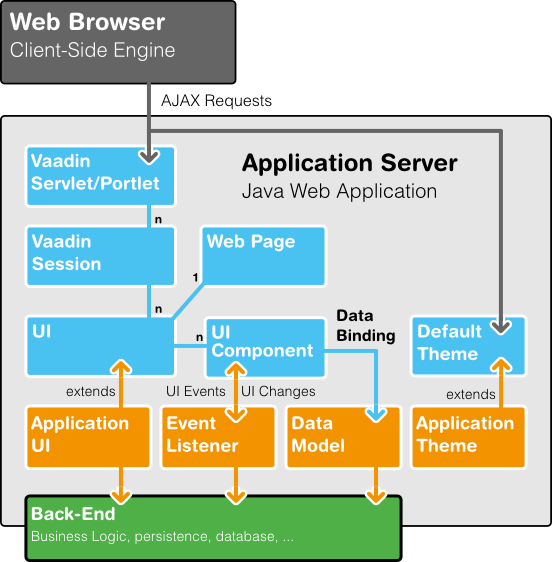
\includegraphics[width=0.7\textwidth]{img/vaadin-arch.png}


\section{Presentation Layer}



\section{Business Logic Layer}


\section{Data Access Layer}



\section{Model Layer}








\end{document}